
\subsection{Single Lepton Top MC Modelling Validation from CR2}
\label{sec:cr2}

IS THIS GOING TO BE DONE WITH A BVETO OR NOT.  IF SO, IS IT GOING TO
BE CSVL OR CSVM?  NEED TO DISCUSS THIS.

The \mt\ tail for single-lepton top events (\ttsl\ and single top) is dominated by jet resolution effects. The \W\ cannot be far off-shell because $\mW < \mtop$.
The modeling of the \mt\ tail from jet resolution effects is studied using \zjets\ data and MC samples. 
\Z\ events are selection by requiring 2 good leptons (satisfying ID and isolation requirements) and requiring the \mll\ to be in the range $81-101$ GeV. 
The negative lepton is treated as a neutrino and so is added to the MET: \met\ $\rightarrow$ \pt(\Lepm) + \met, 
and the \mt\ is recalculated with the positive lepton \mt(\Lepp, \met).
The resulting ``pseudo-\mt'' is dominated by jet resolution effects, since no off-shell 
\Z\ production enters the sample due to the \mll\ requirement.
This section describes how well the MC predicts the tail of ``pseudo-\mt''. 

The underlying distributions are shown in Fig.~\ref{fig:cr2met}
and~\ref{fig:cr2mtrest}.  The comparison of data and MC event counts 
is shown in Table~\ref{tab:cr2yields}.  From this table we extract
the data to MC scale factors $SFR^{e}_{top}$ and  $SFR^{\mu}_{top}$. 


\begin{table}[!h]
\begin{center}
{\footnotesize
\begin{tabular}{l||c|c||c|c|c|c|c}
\hline
Sample              & CR2PRESEL0 &CR2PRESEL1 & CR2A & CR2B & CR2C &
CR2D & CR2E\\
\hline
\hline
DY MC 		  & $27 \pm 2$ & $23 \pm 2$ & $14 \pm 2$ & $25 \pm 3$ & $11 \pm 2$ & $3 \pm 1$ & $1 \pm 1$ \\
Data - non-DY MC 	  & $47 \pm 8$ & $36 \pm 7$ & $28 \pm 6$ & $35 \pm 6$ & $19 \pm 5$ & $11 \pm 3$ & $1 \pm 1$ \\
\hline
Data/MC SF: ($SFR_{top}$) 	  & $1.75 \pm 0.31$ & $1.58 \pm 0.32$ & $2.00 \pm 0.47$ & $1.38 \pm 0.31$ & $1.78 \pm 0.56$ & $3.29 \pm 1.73$ & $0.98 \pm 1.20$ \\
\hline
\end{tabular}}
\caption{ Yields in \mt\ tail comparing the \zjets\ MC prediction (after
  applying SFs) to data after subtracting the non-\zjets\ components. 
  CR2PRESEL refers to a sample with $\met>50$ GeV and $\mt>150$ GeV.
  The uncertainties are statistical only.  NEED TO ADD THE SYMBOLS
  DEFINED IN THE TEXT FOR THESE SCALE FACTORS.  IS THIS GOING TO BE
  DONE SEPARATELY FOR MUONS AND ELECTRONS???
  MAYBE WANT TO REMOVE LAST ENTRIES WHERE STATS ARE VERY LOW
\label{tab:cr2zyields}}
\end{center}
\end{table}


\begin{table}[!h]
\begin{center}
{\footnotesize
\begin{tabular}{l||c|c||c|c|c|c|c}
\hline
Sample              & CR2PRESEL0 &CR2PRESEL1 & CR2A & CR2B & CR2C &
CR2D & CR2E\\
\hline
\hline
MC 		  & $36 \pm 2$ & $30 \pm 2$ & $18 \pm 1$ & $30 \pm 2$ & $13 \pm 1$ & $5 \pm 0$ & $2 \pm 0$ \\
Data 		  & $56$ & $43$ & $32$ & $40$ & $21$ & $12$ & $2$ \\
\hline
Data/MC SF: ($SFR_{top}$) 	  & $1.56 \pm 0.23$ & $1.44 \pm 0.24$ & $1.77 \pm 0.34$ & $1.32 \pm 0.22$ & $1.65 \pm 0.37$ & $2.65 \pm 0.79$ & $0.99 \pm 0.71$ \\
\hline
\end{tabular}}
\caption{ Yields in \mt\ tail comparing the MC prediction (after
  applying SFs) to data. CR2PRESEL refers to a sample with $\met>50$
  GeV and $\mt>150$ GeV.
  The uncertainties are statistical only.  NEED TO ADD THE SYMBOLS
  DEFINED IN THE TEXT FOR THESE SCALE FACTORS.  IS THIS GOING TO BE
  DONE SEPARATELY FOR MUONS AND ELECTRONS???
  MAYBE WANT TO REMOVE LAST ENTRIES WHERE STATS ARE VERY LOW
\label{tab:cr2yields}}
\end{center}
\end{table}



\begin{figure}[hbt]
  \begin{center}
%	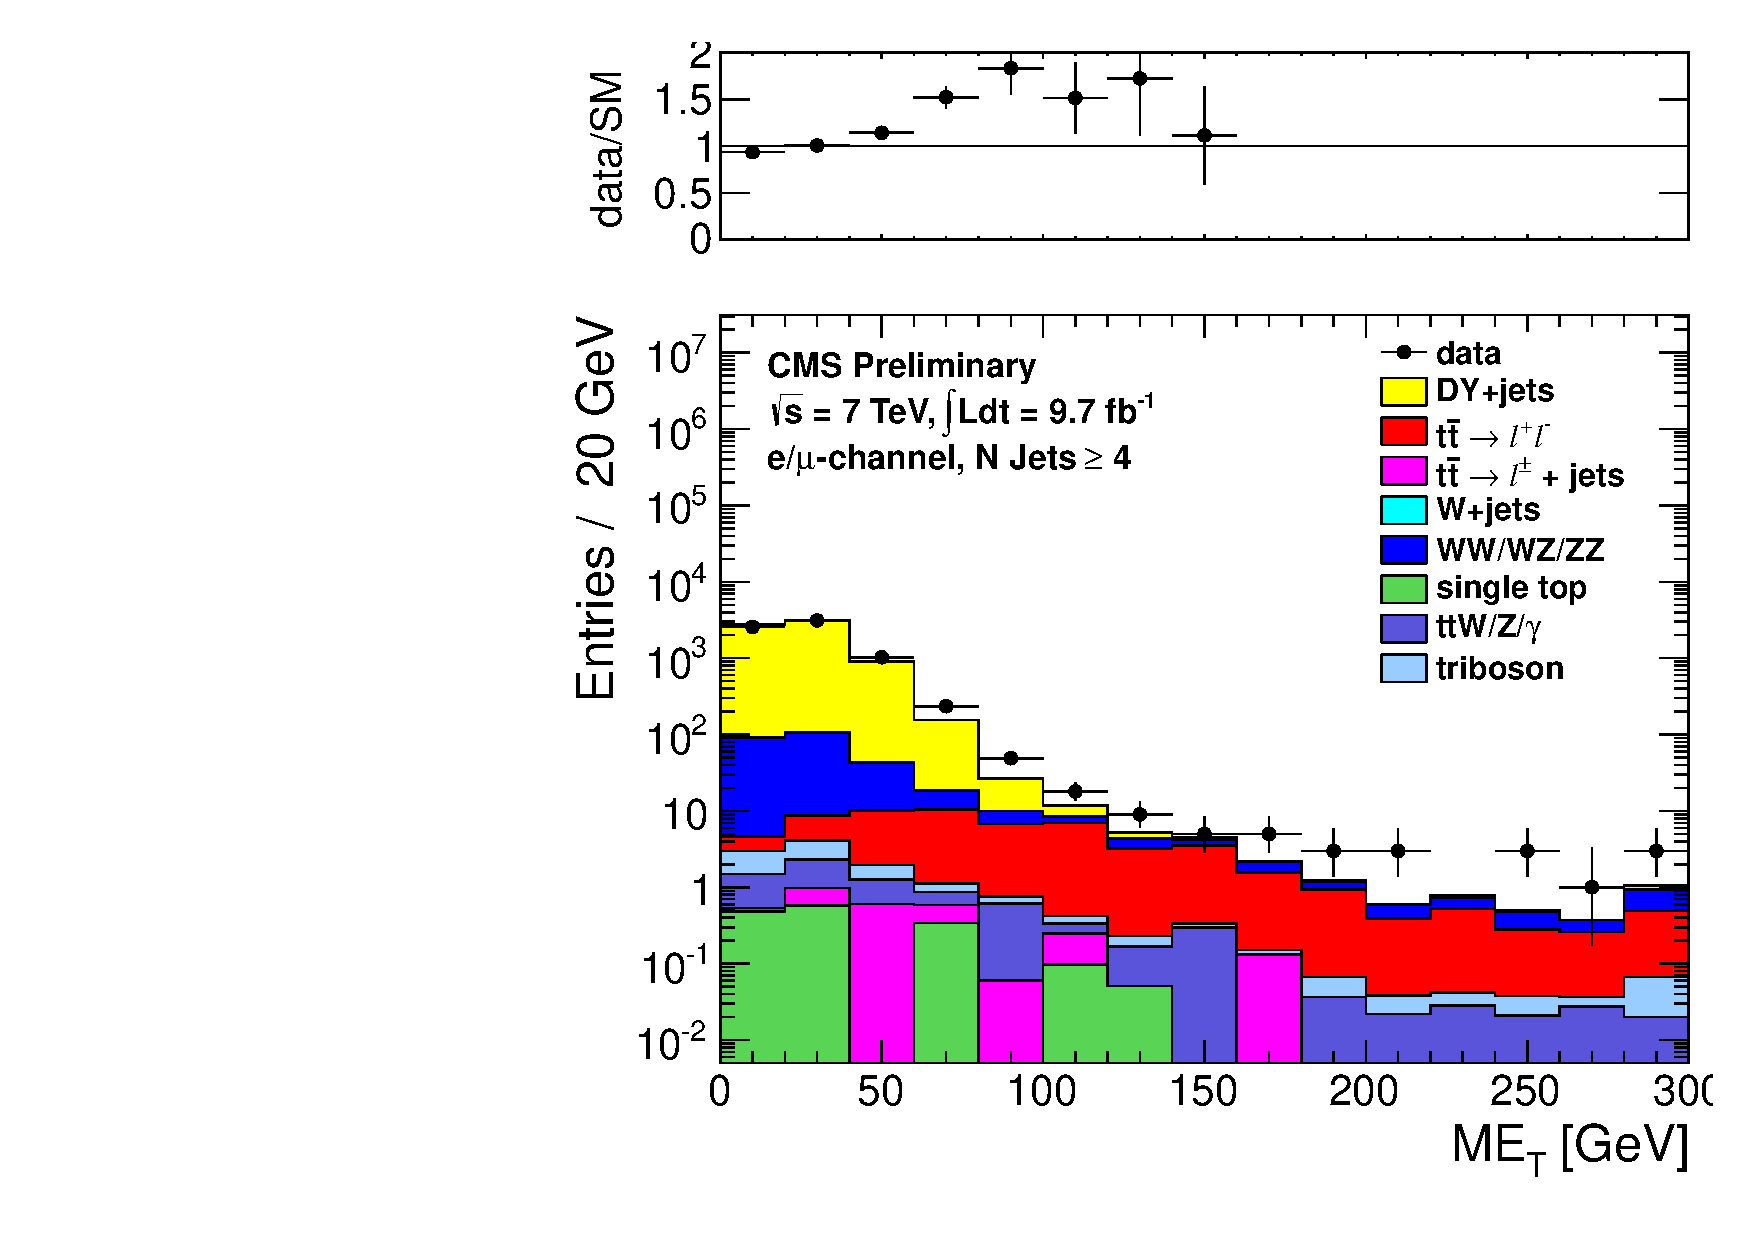
\includegraphics[width=0.5\linewidth]{plots/CR2plots/met_scaled_nj4_emucomb.pdf}%
	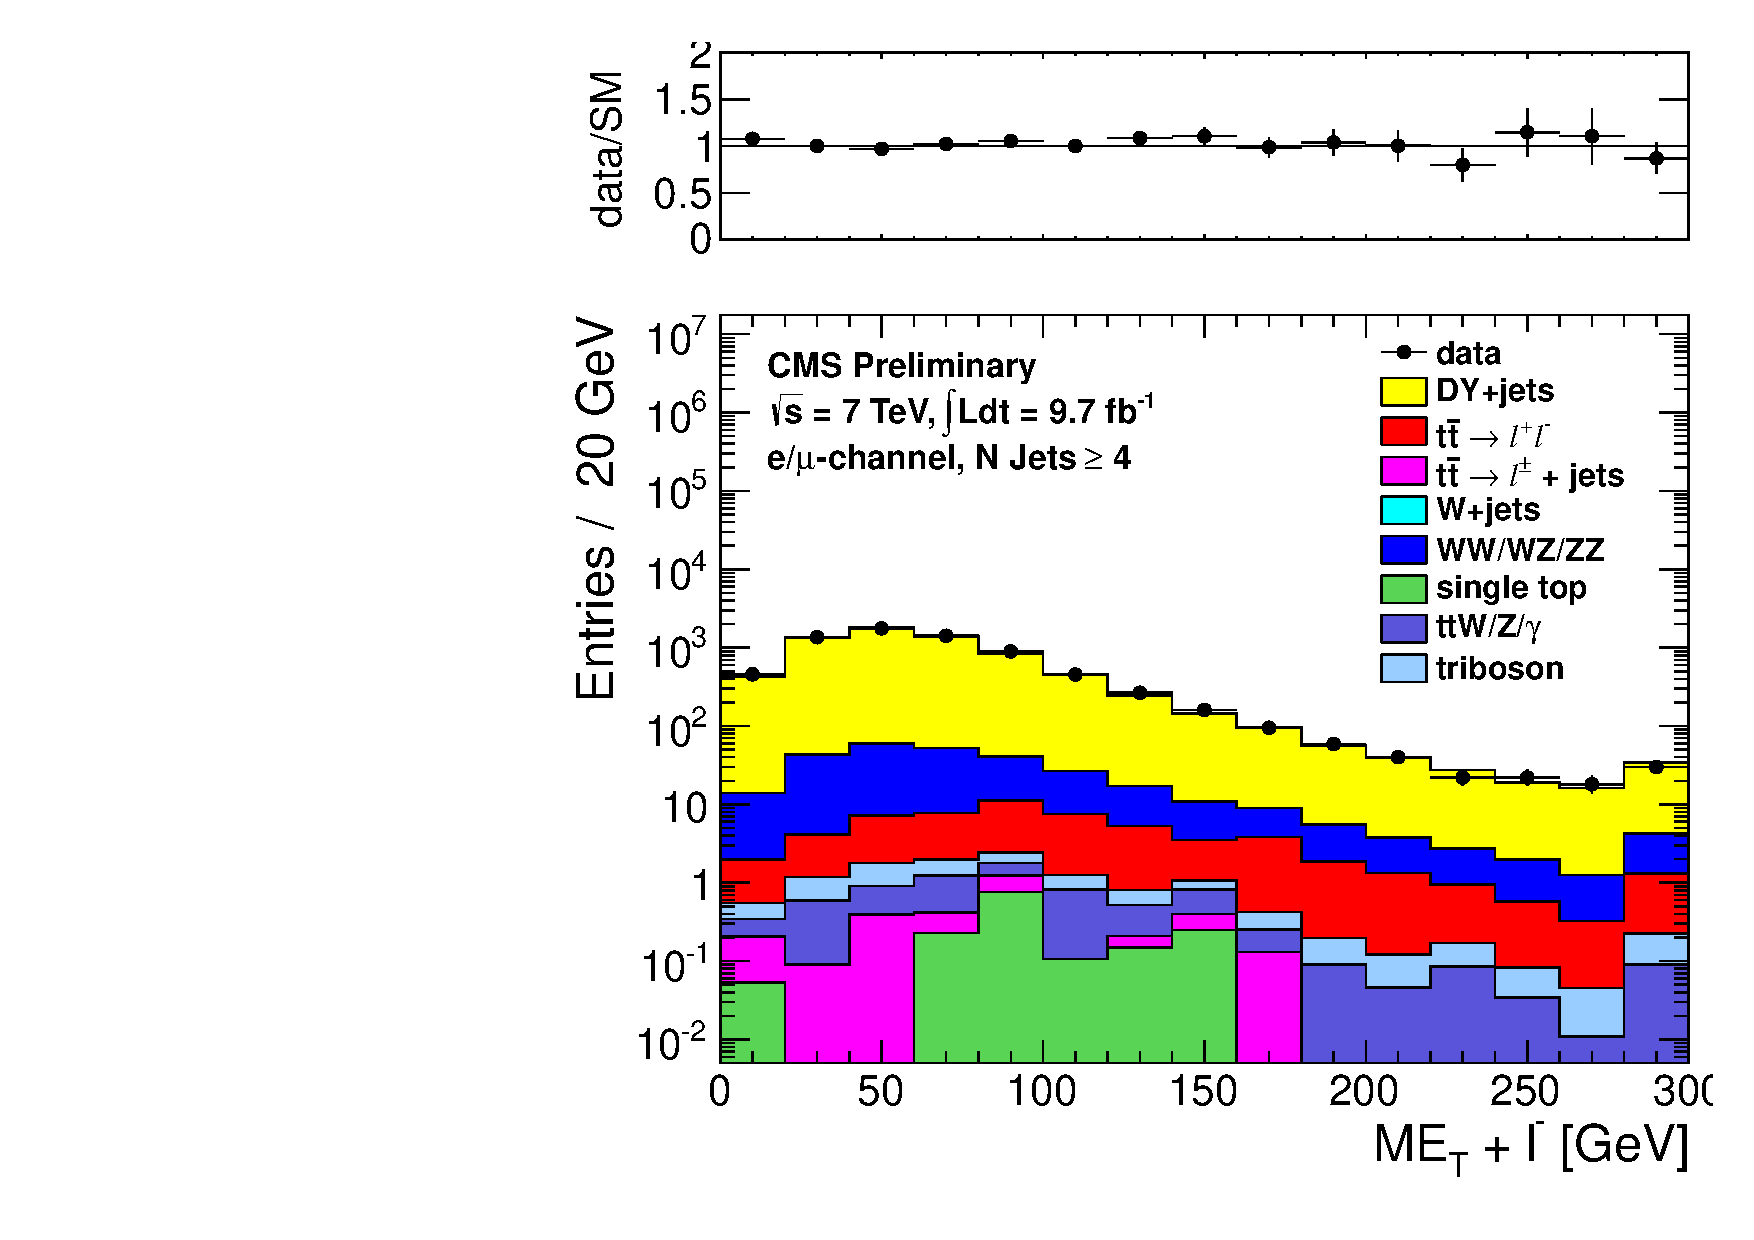
\includegraphics[width=0.5\linewidth]{plots/CR2plots/met_lepcor_scaled_nj4_emucomb.pdf}%
	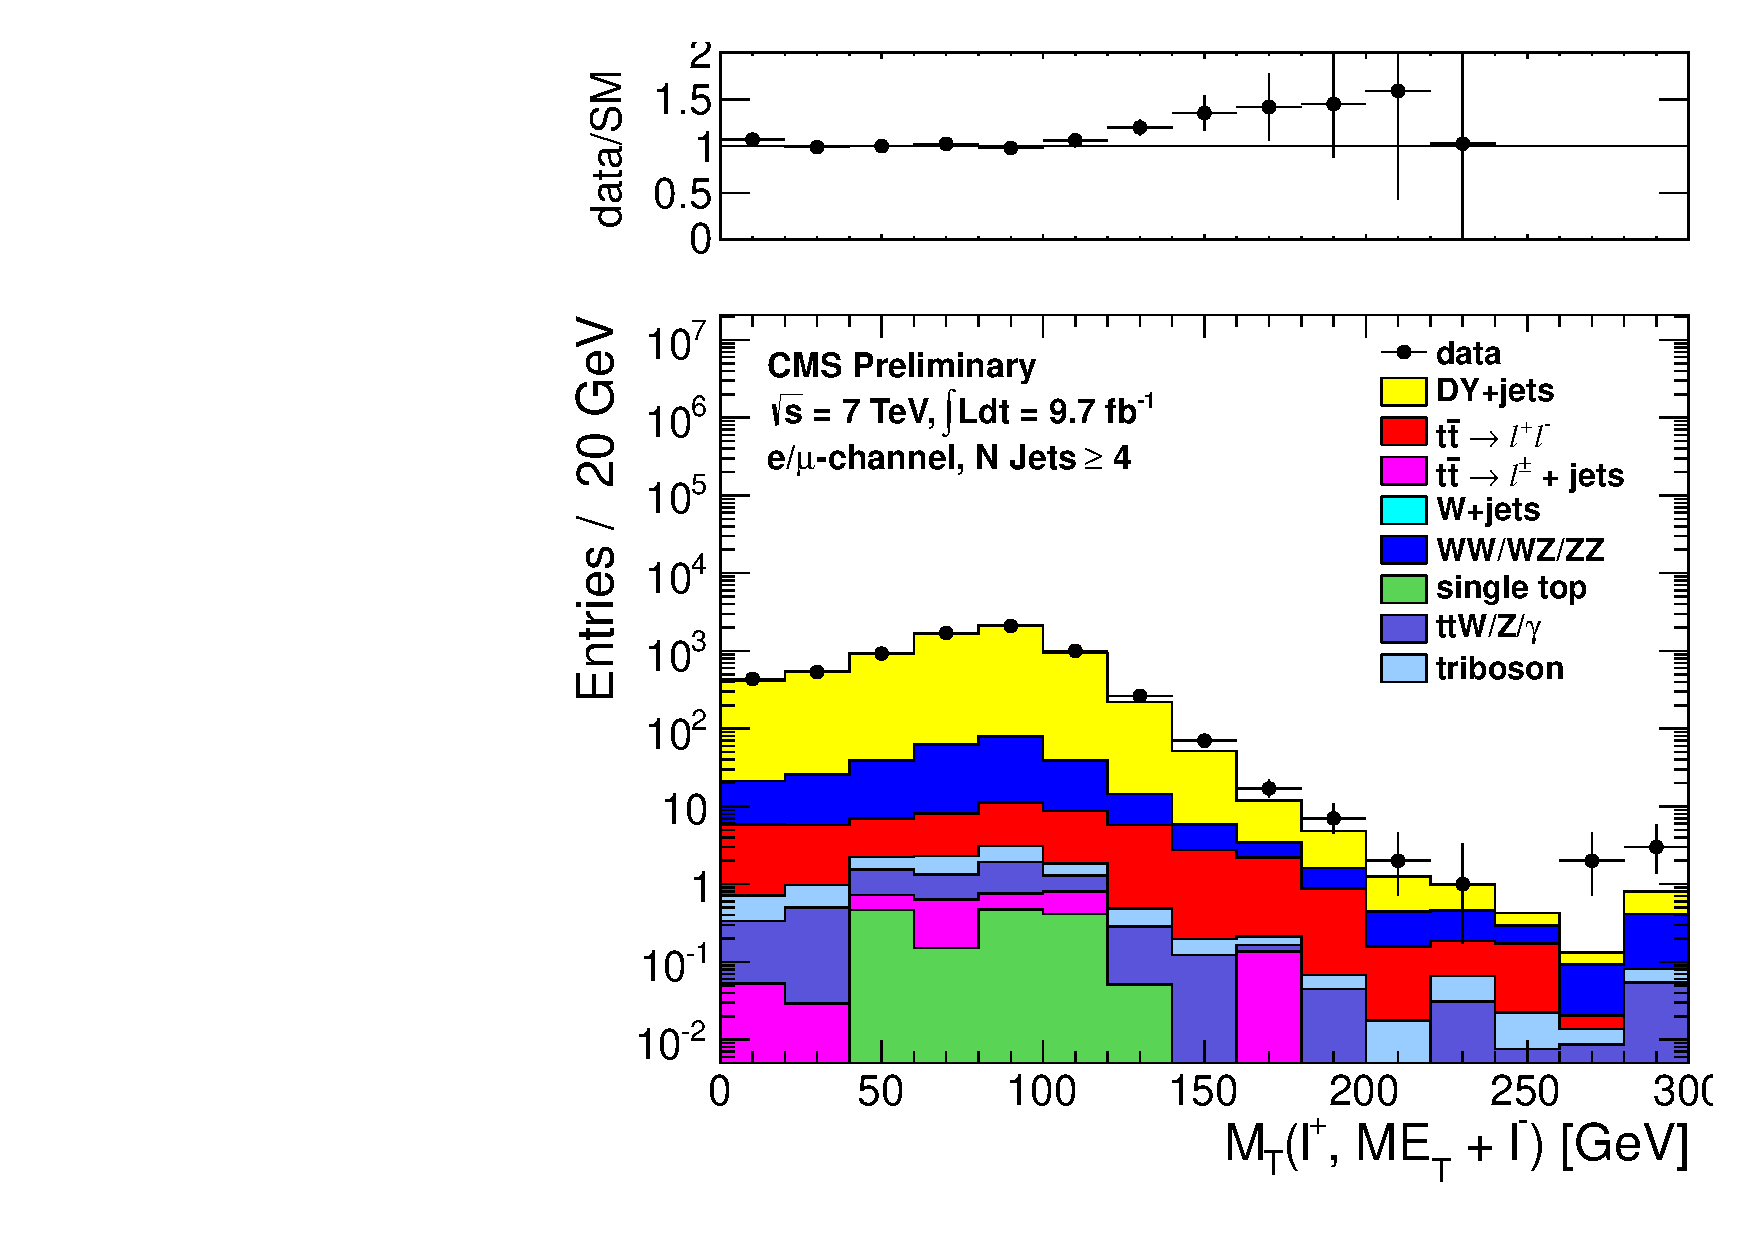
\includegraphics[width=0.5\linewidth]{plots/CR2plots/mt_lepcor_scaled_nj4_emucomb.pdf}
	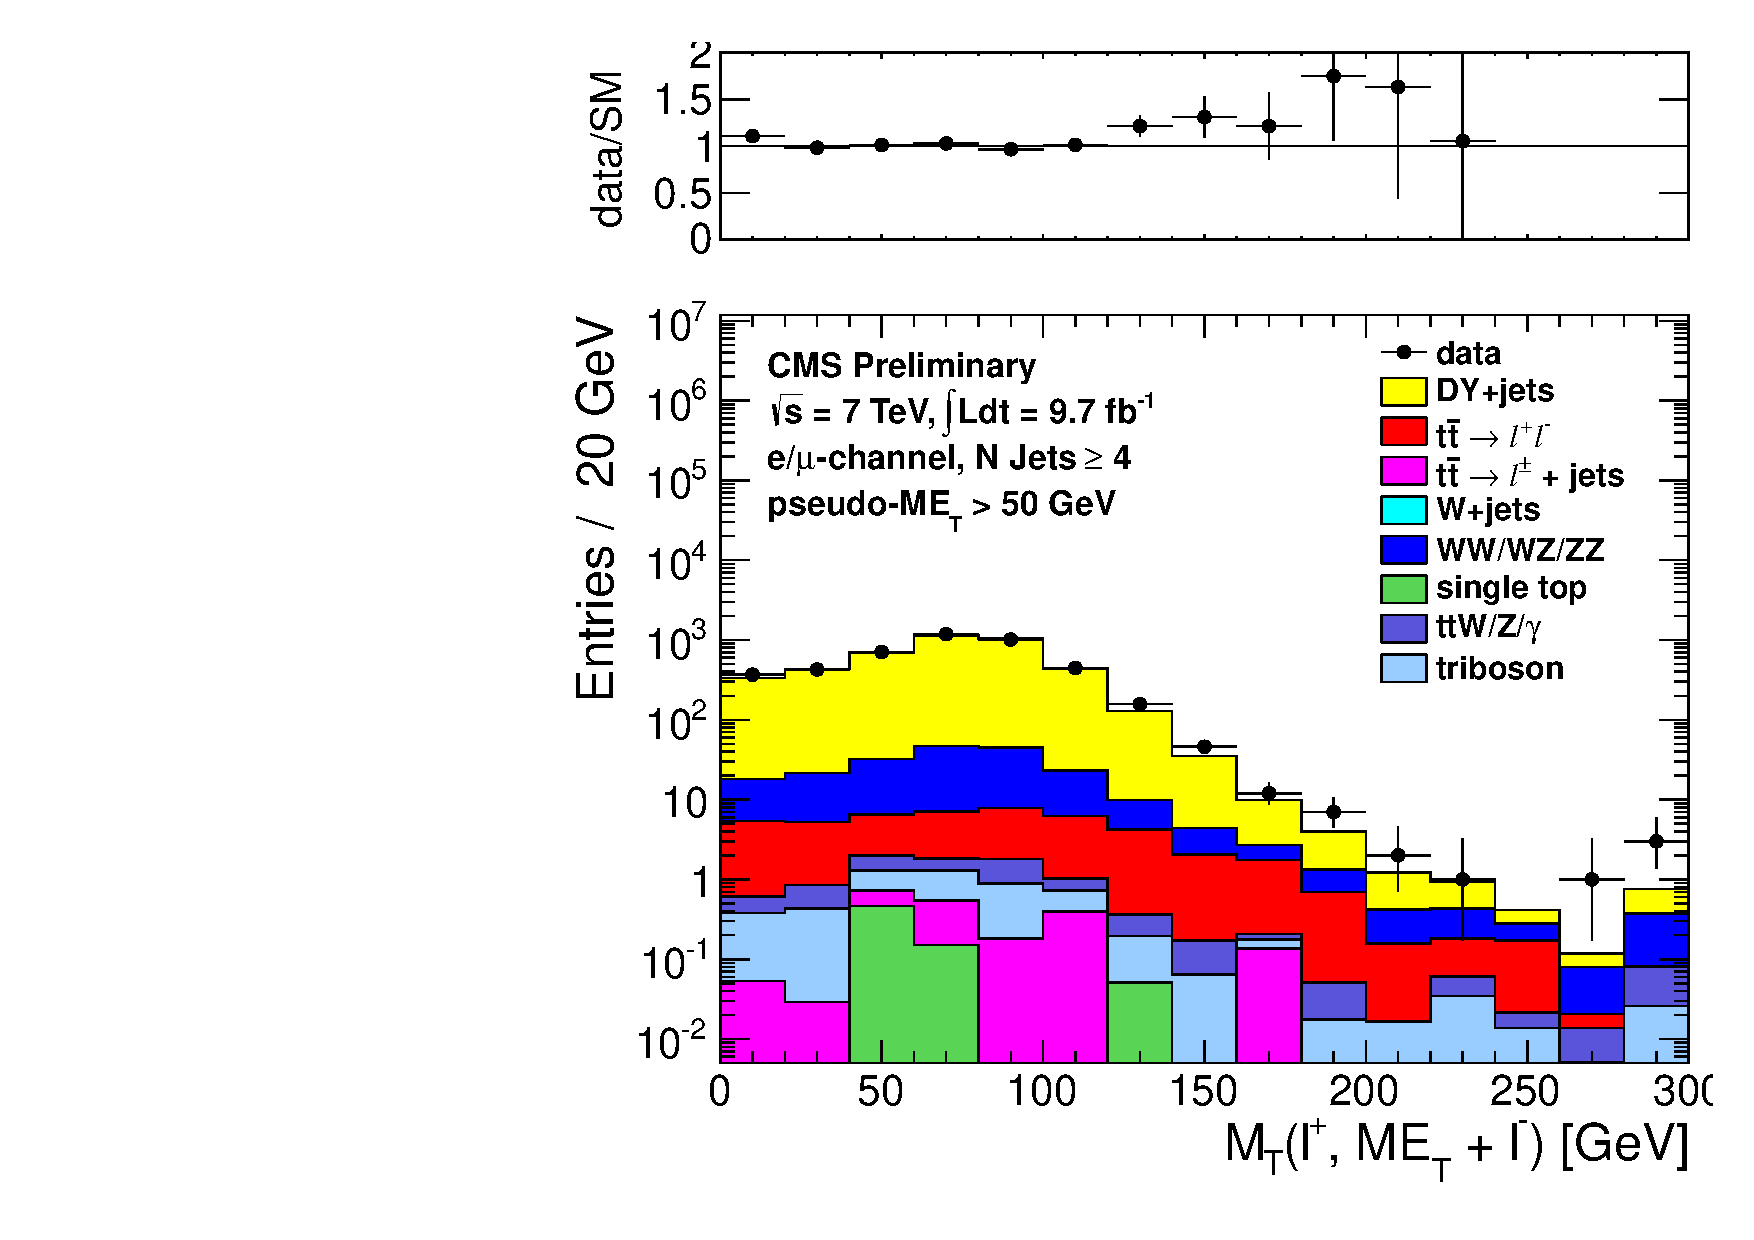
\includegraphics[width=0.5\linewidth]{plots/CR2plots/mt_lepcor_scaled_met50_nj4_emucomb.pdf}%
	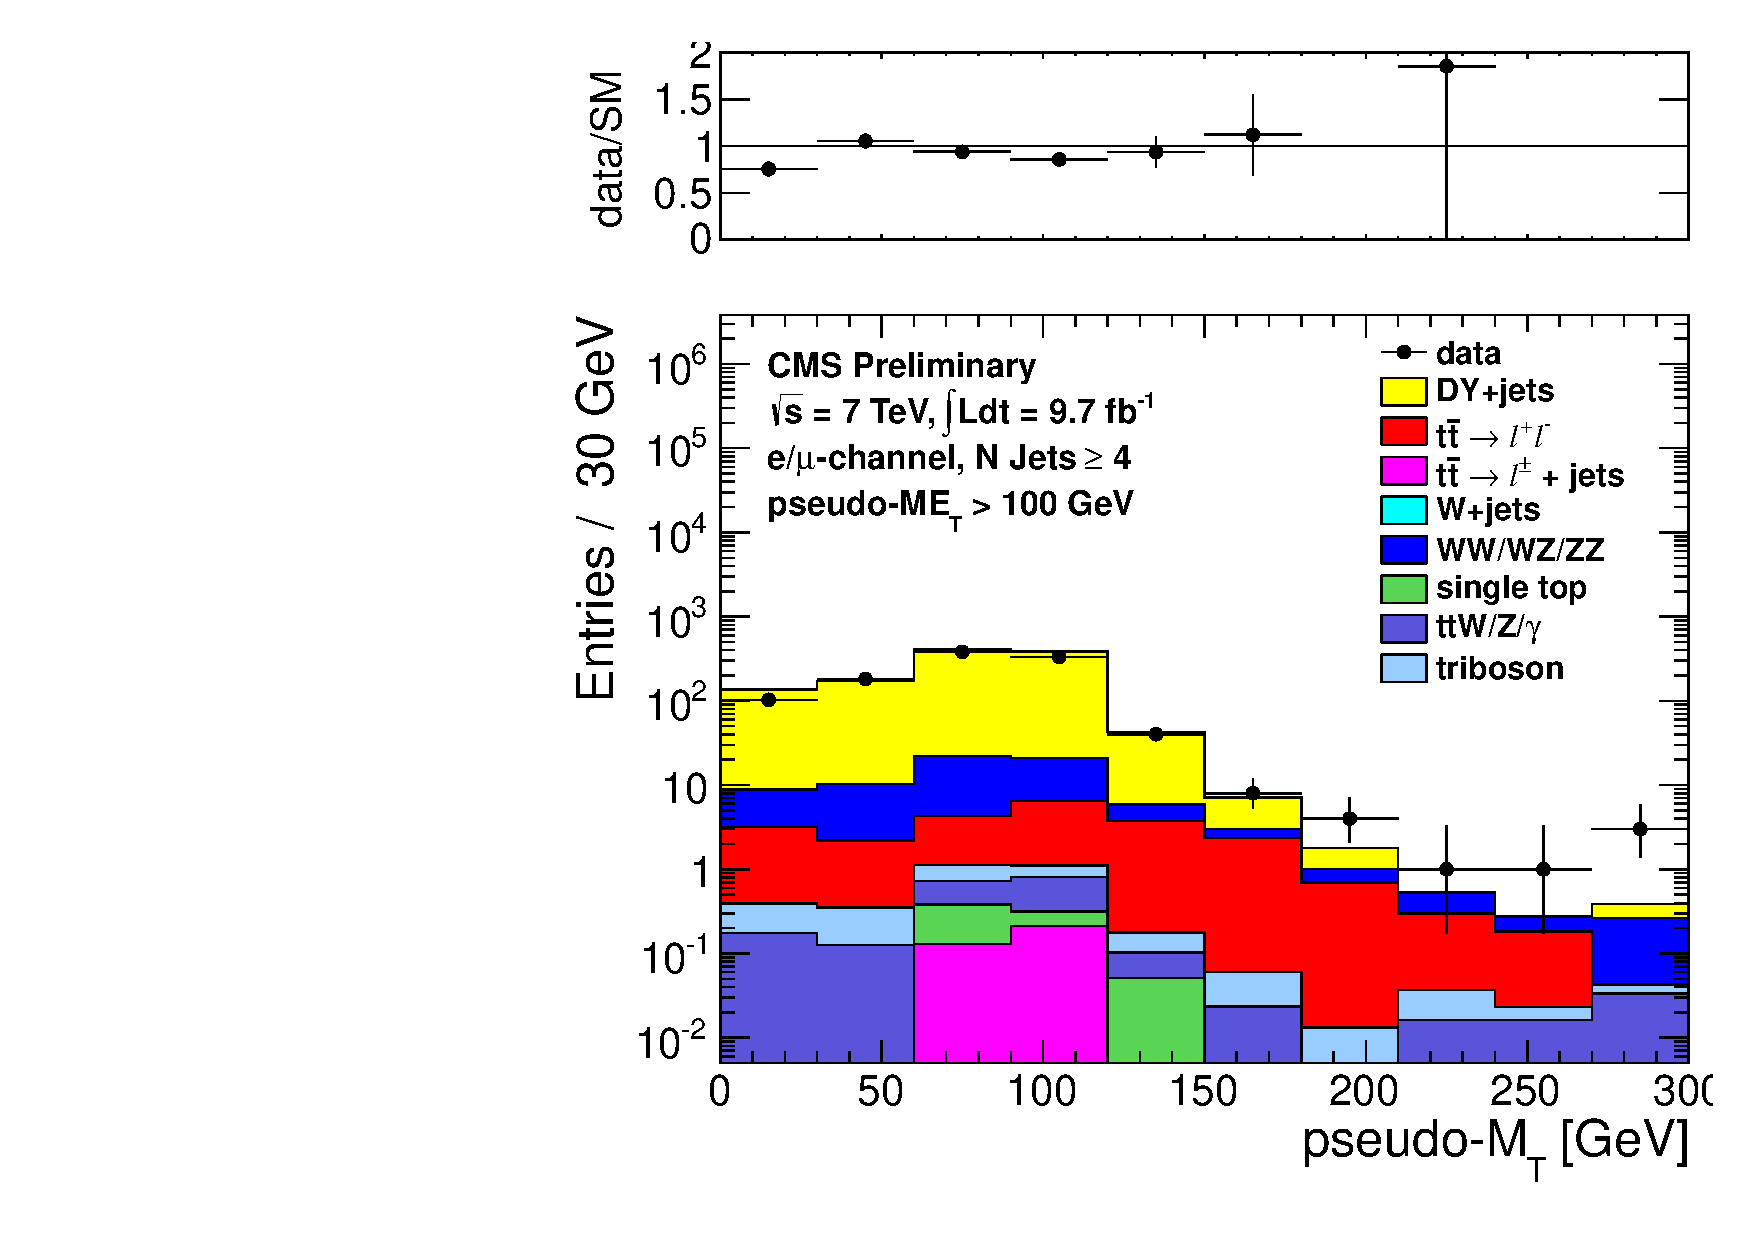
\includegraphics[width=0.5\linewidth]{plots/CR2plots/mt_lepcor_scaled_met100_nj4_emucomb.pdf}

    \caption{
      Comparison of the pseudo\-\met\ (top, left), pseudo\-\mt\ (top,
      right and bottom) distributions in data vs. MC for events
      satisfying the requirements of CR2, combining both the muon and
      electron channels. The pseudo\-\mt\ distributions are shown
      before any additional requirements (top, right) and after
      requiring pseudo\-\met>50 GeV (bottom, left) and pseudo\-\met>100 GeV (bottom, right) .
\label{fig:cr2met} 
}  
      \end{center}
\end{figure}

\begin{figure}[hbt]
  \begin{center}
	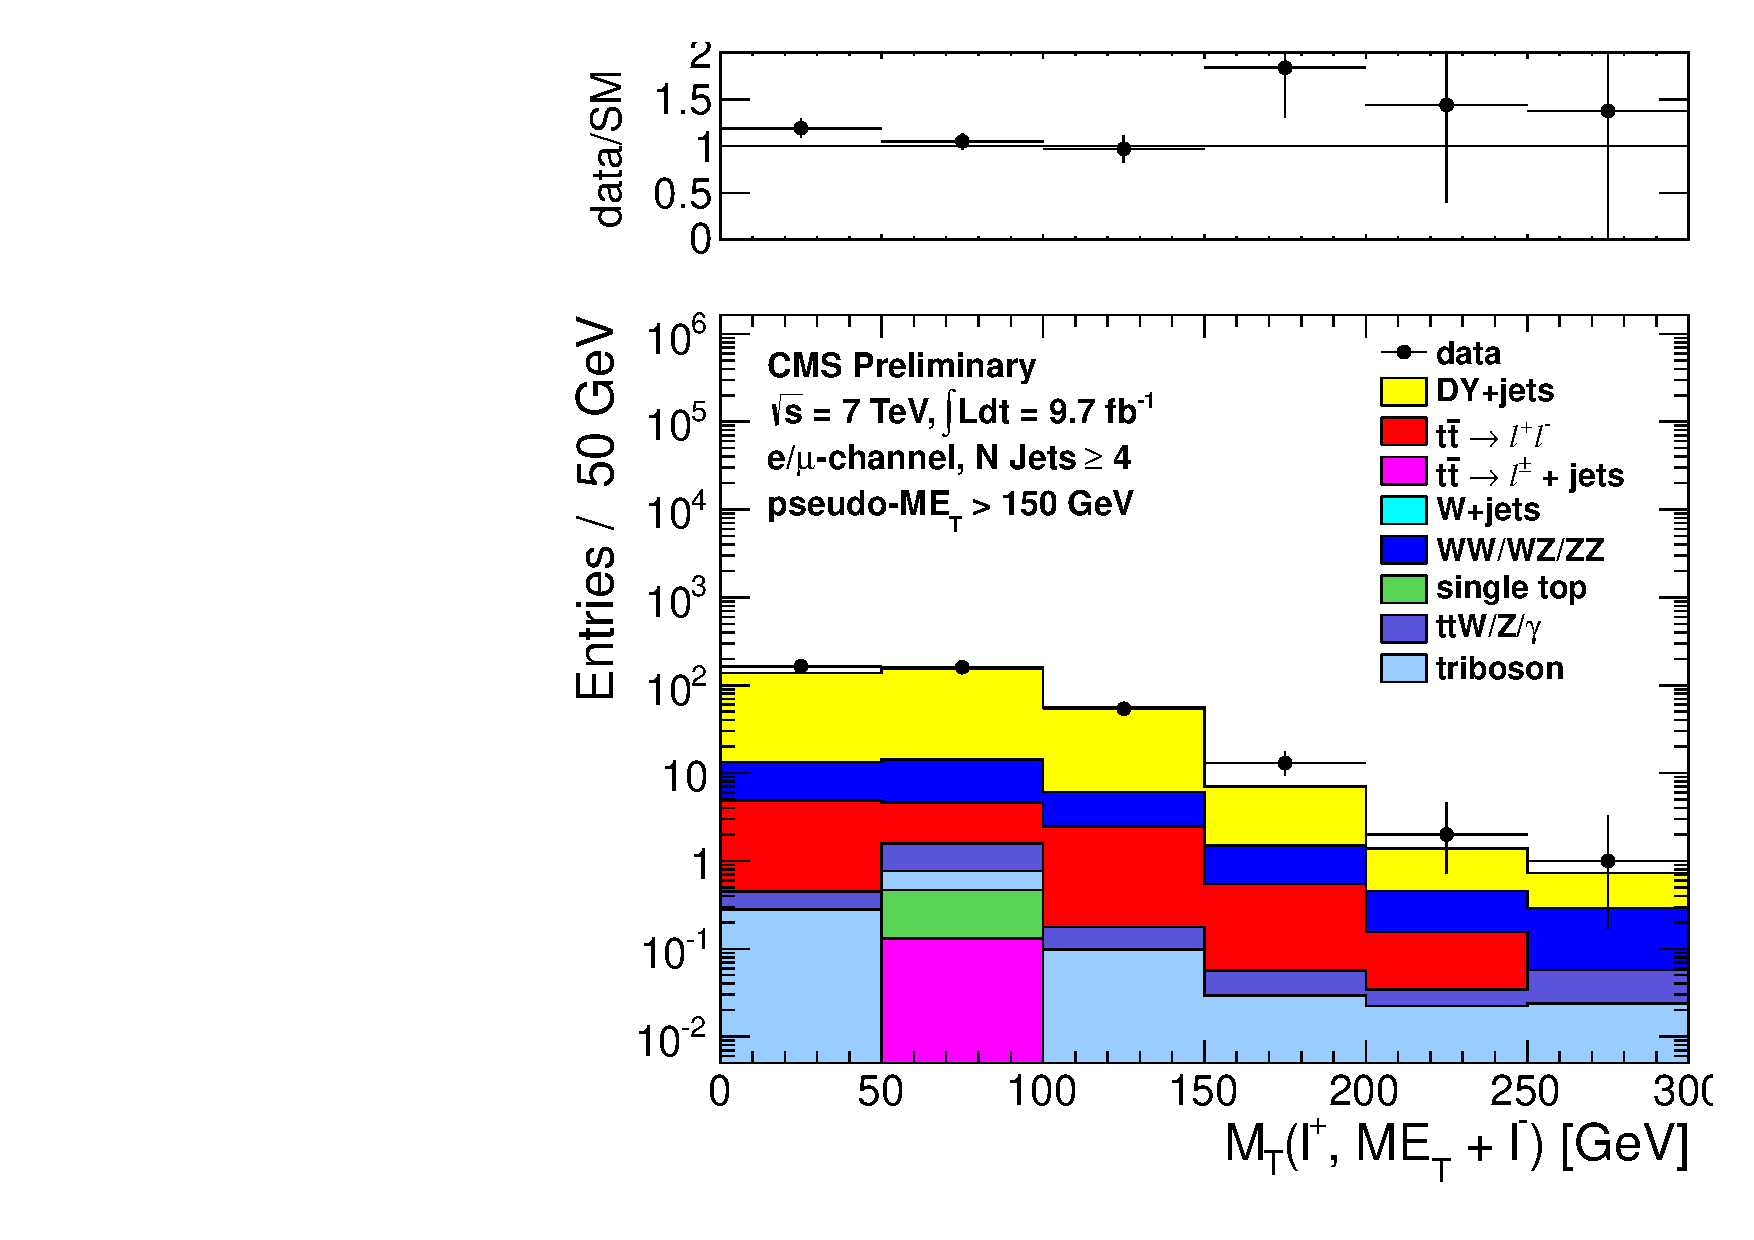
\includegraphics[width=0.5\linewidth]{plots/CR2plots/mt_lepcor_scaled_met150_nj4_emucomb.pdf}%
	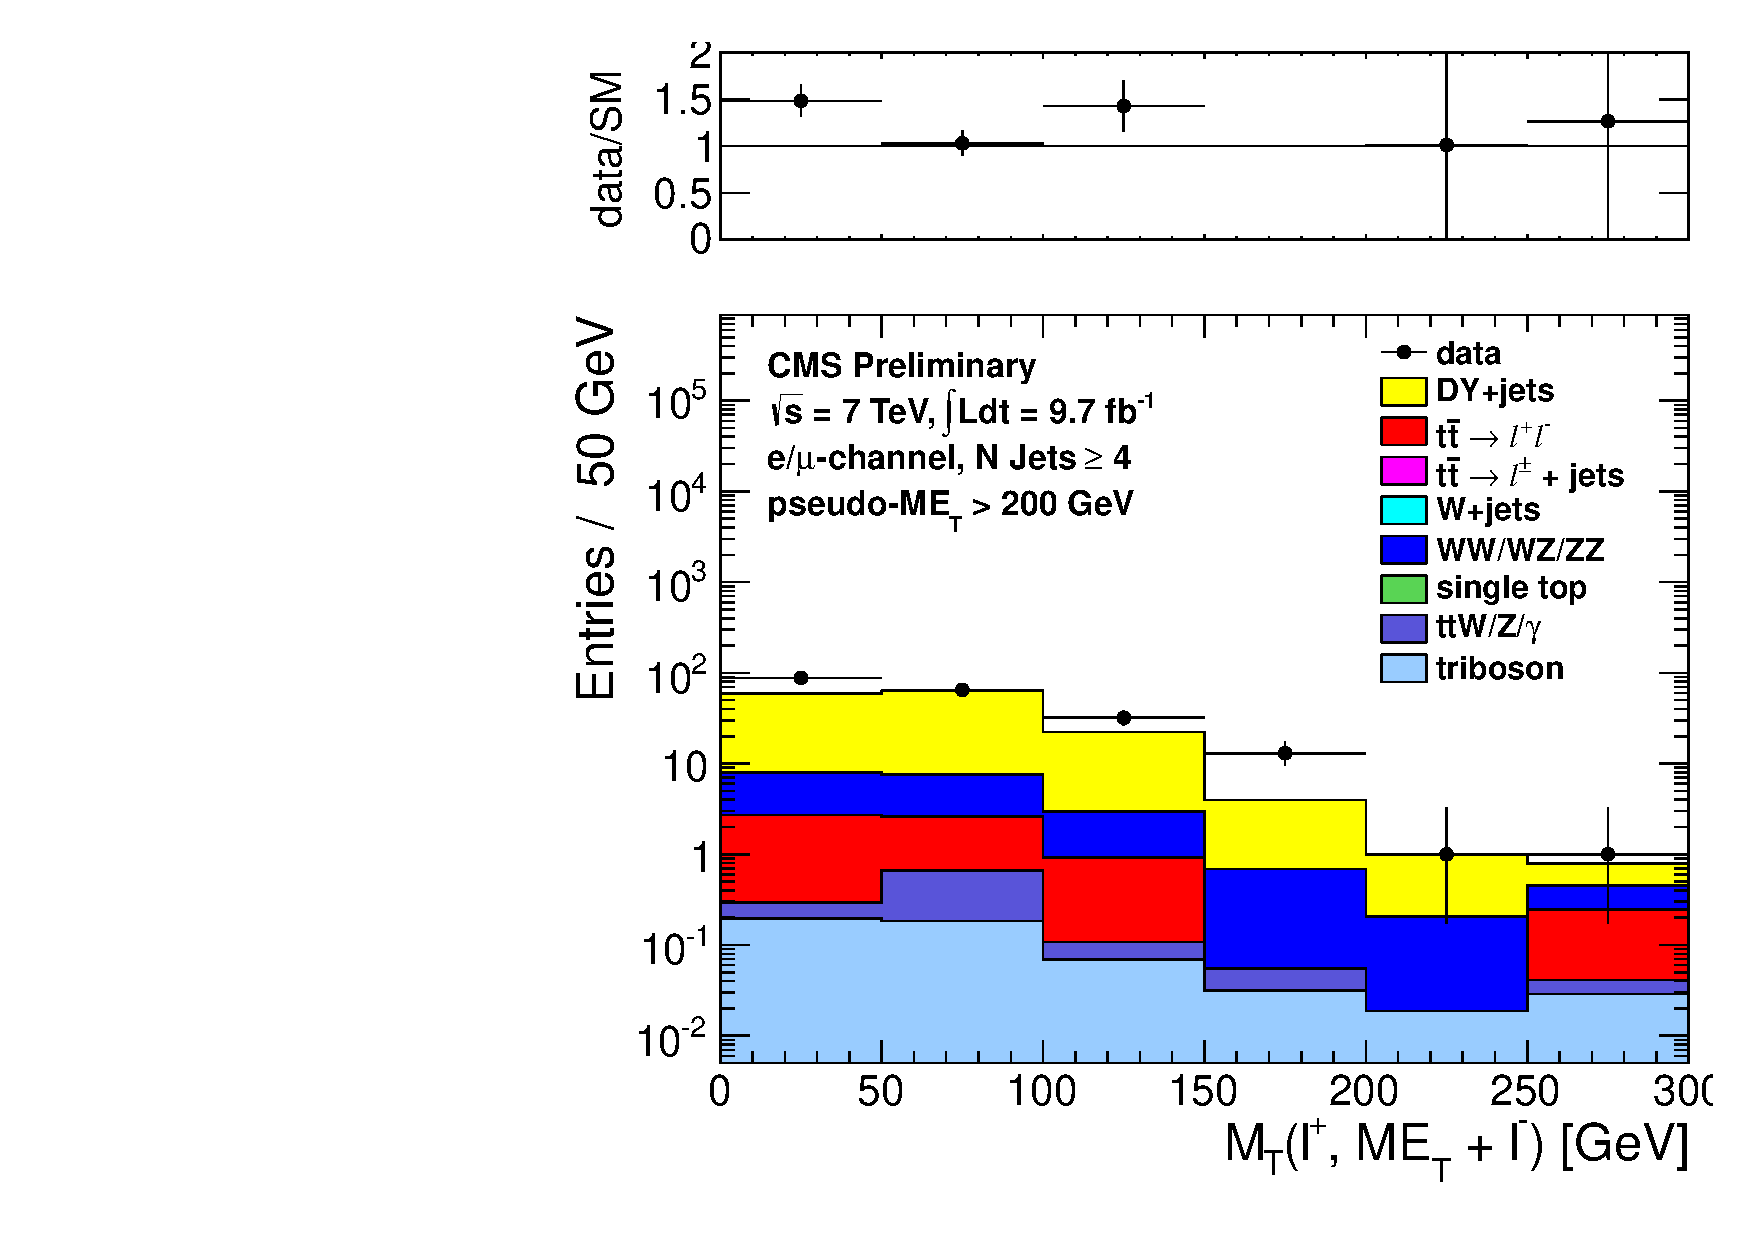
\includegraphics[width=0.5\linewidth]{plots/CR2plots/mt_lepcor_scaled_met200_nj4_emucomb.pdf}
	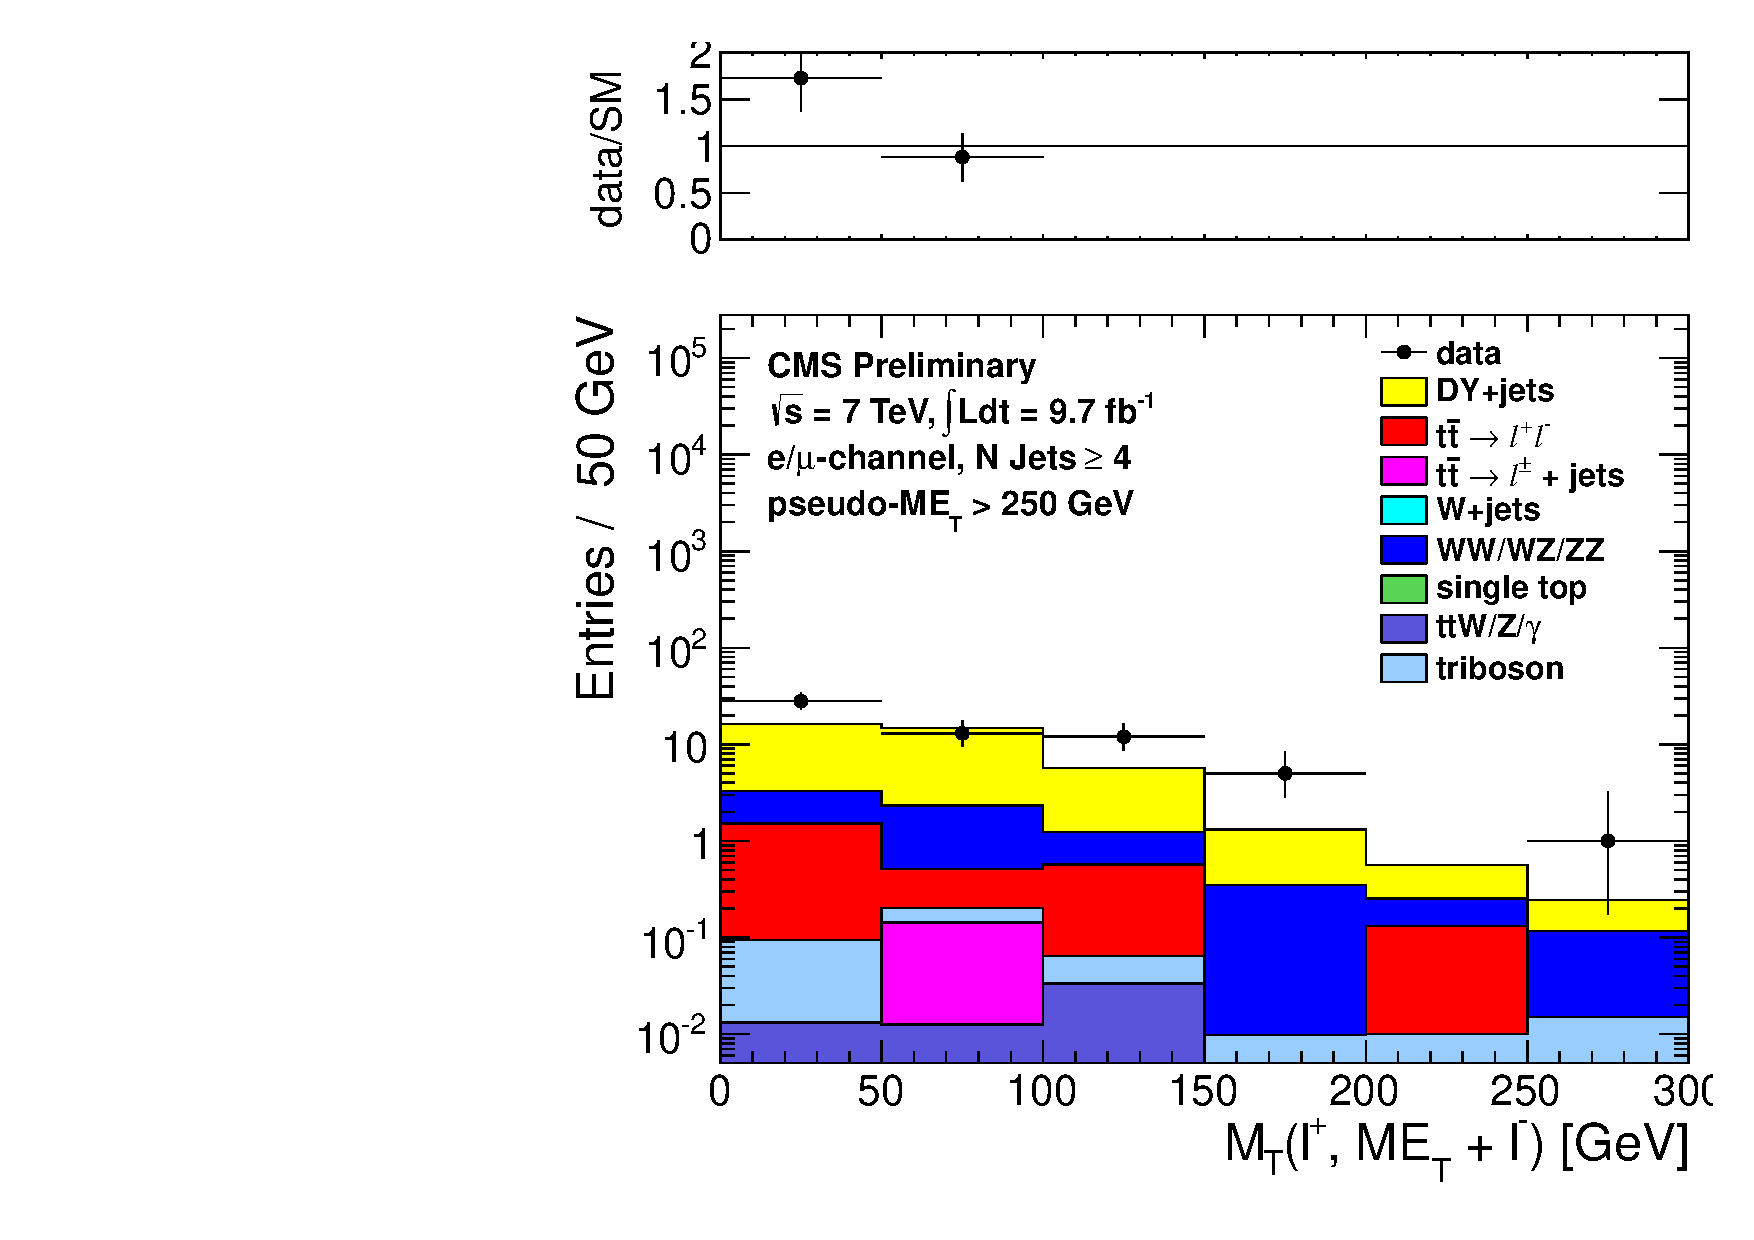
\includegraphics[width=0.5\linewidth]{plots/CR2plots/mt_lepcor_scaled_met250_nj4_emucomb.pdf}%
	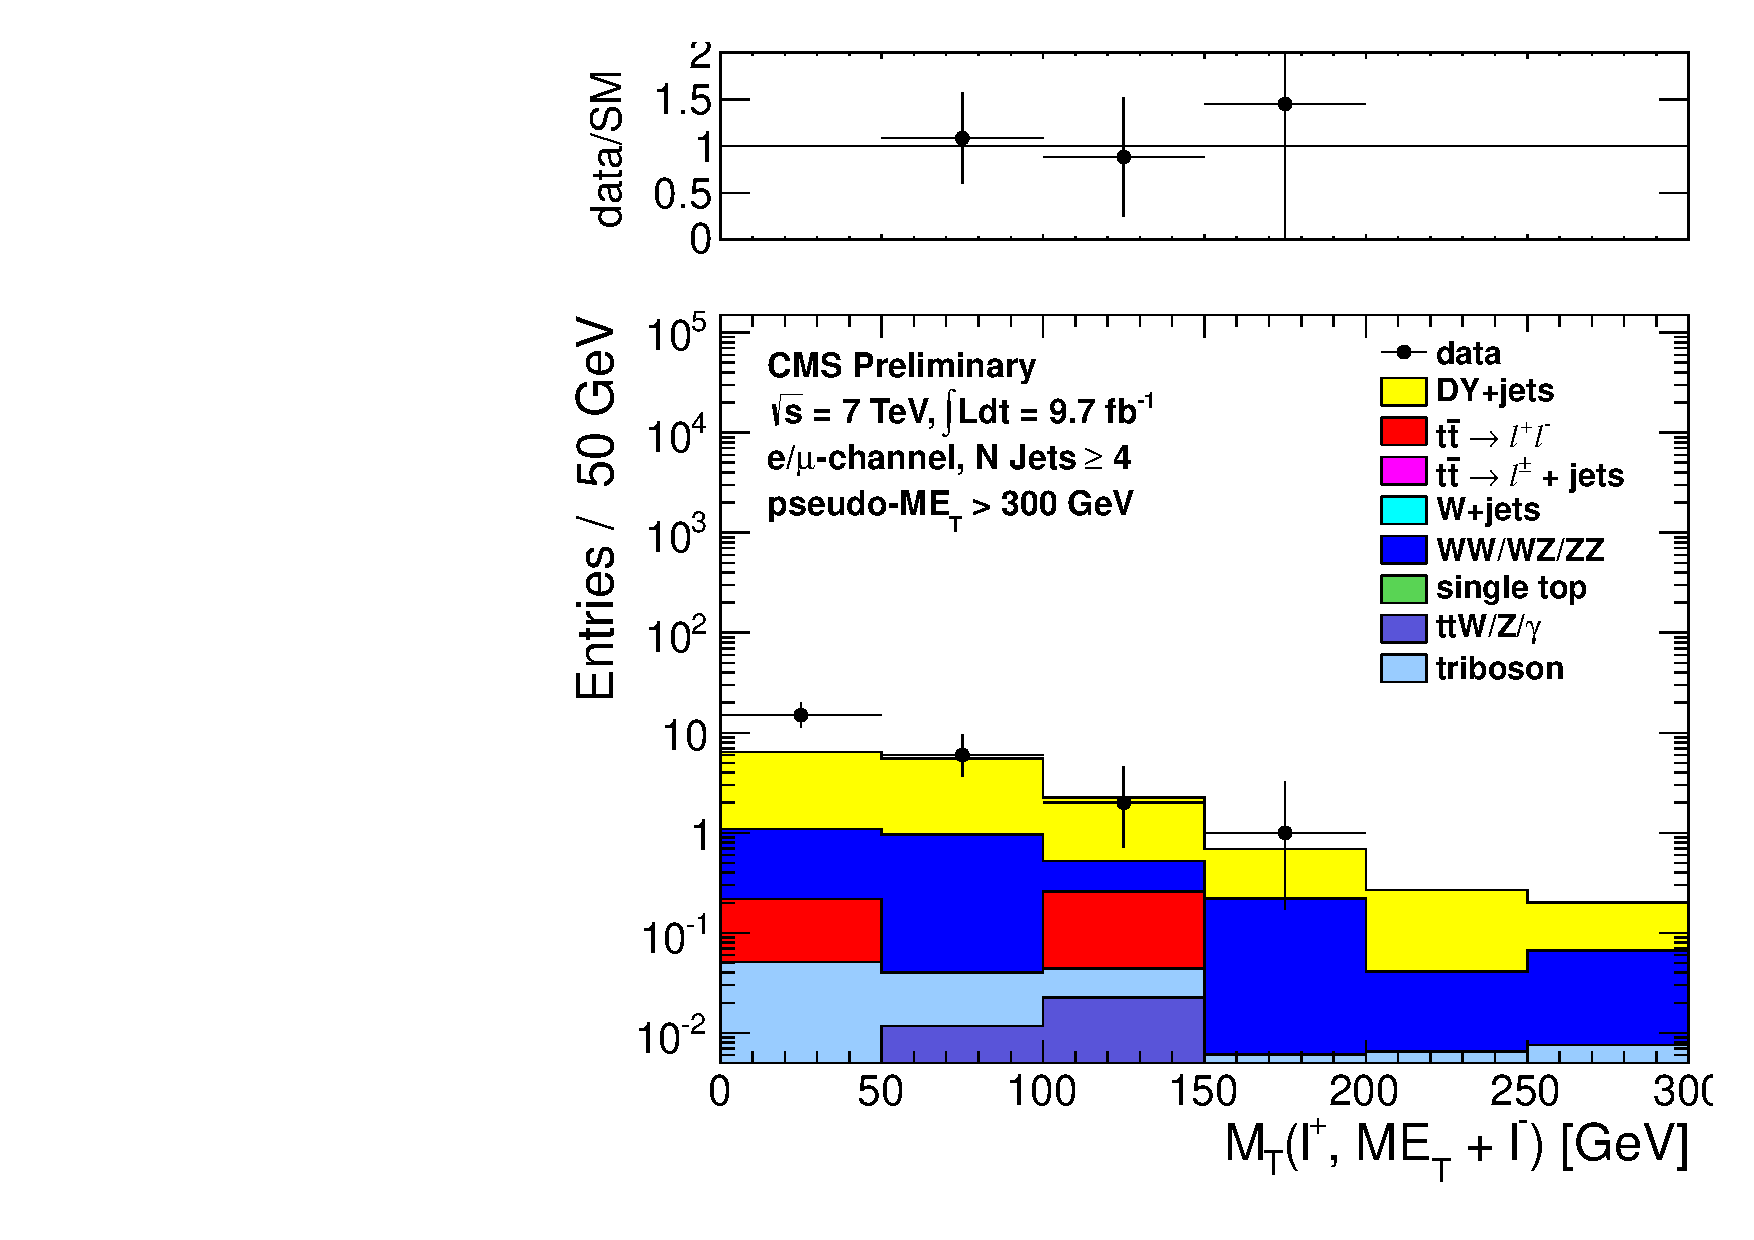
\includegraphics[width=0.5\linewidth]{plots/CR2plots/mt_lepcor_scaled_met300_nj4_emucomb.pdf}
    \caption{
      Comparison of the \mt\ distribution in data vs. MC for events
      satisfying the requirements of CR2, combining both the muon and
      electron channels. The pseudo-\met\ requirements used are
      150 GeV (top, left), 200 GeV (top, right), 250 GeV (bottom,
      left) and 300 GeV (bottom, right).
\label{fig:cr2mtrest} 
}  
      \end{center}
\end{figure}
\clearpage